

\section{Aim}
This document presents a conformal mapping approach to evaluating potential function derivatives in two dimensions at a modulated free surface.
The problem is encountered within free-surface hydrodynamics whence boundary conditions require a vertical velocity component $v=\phi_y$ evaluated at the free surface $(\x,\surf(\x))$ itself.
A standard approach for such an evaluation, e.g.\ adopted in numerical higher order spectral methods, is to related the free surface $\y=\surf$ to the horizontal line $\y=0$ through Taylor expansions.
The downside of such an approach is that the Taylor series convergence is limited \citep{west1981deep} and that it requires evaluation of a number of functional derivatives.
The number is proportional to the square of the expansion order, each requiring a pair of Fourier transformations.
\\

As will be shown, the conformal mapping approach presented here provides and explicit expression for the surface velocities for a given surface potential.
The expression does not entail any series expansions and is not subject to convergence limitations.
What's more, it requires only four Fourier transformations---the surface potential and elevation, for the surface elevation gradient and for the final vertical velocity component.

\section{Derivation}
Assume surface elevation $\surf(\x)$ and surface potential $\phi\S(\x)$ known.

In complex coordinates
\[  \z = \x+\ii\y \]
of the physical plane
we introduce the conformal map
\begin{equation}
\z\mapsto\zmap(\zz) = \zz + \ii \sum_{j=-\infty}^\infty\h\surf_j \ee^{\ii k_j \zz}
\label{eq:map}
\end{equation}
where $\h\surf_j$ are the Fourier components of the surface elevation, i.e.,\
\[
\surf(\x) = \sum_{j=-\infty}^\infty\h\surf_j \ee^{\ii k_j \x}.
\]
We use $\xx$ and $\yy$ respectively for the real and imaginary components of $\zz$; $\zz = \xx+\ii\yy$.
Notice that 
\begin{equation}
\zmap(\xx) = \xx+\ii \surf(\xx),
\label{eq:mapXi}
\end{equation}
i.e., $\zmap$ vartically  maps the zero-line $\zz=\xx$ onto the free surface $\z=\x+\ii\eta(\x)$.
Conversely,
\begin{equation}
\zzmap(\x+\ii\surf) = \x.
\label{eq:invMap}
\end{equation}
An sketch is given in \autoref{fig:map} with an example for a single harmonic in \autoref{fig:mapReg}.


\begin{figure}[h!ptb]%
\center
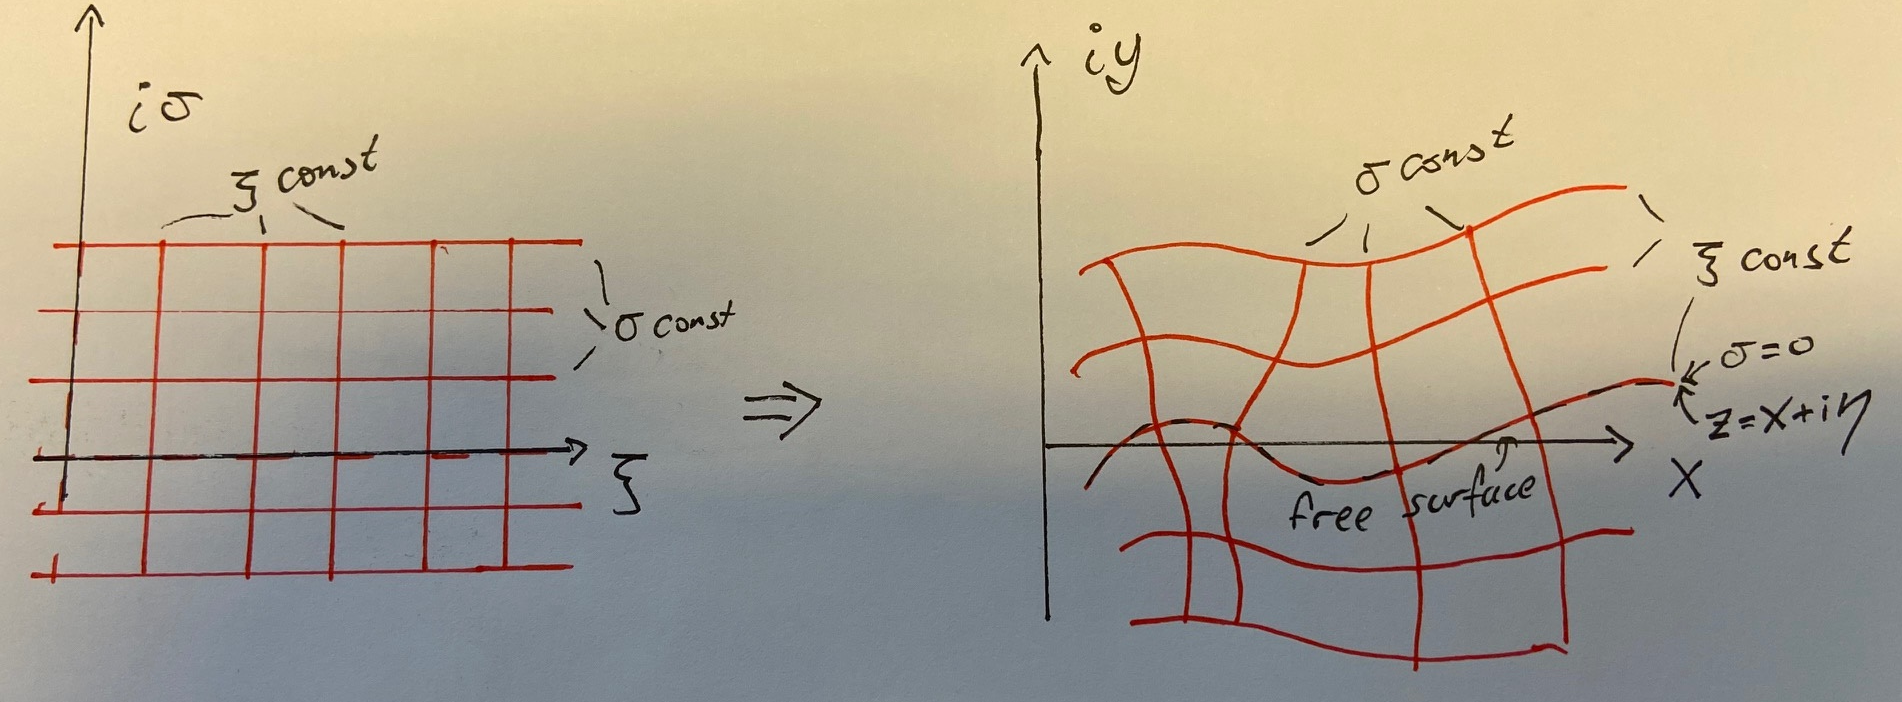
\includegraphics[width=.75\columnwidth]{./figures/map.png}%
\caption{Conformal map, mapping line $\yy=0$ to the free surface $\y=\surf$.}%
\label{fig:map}%
\end{figure}
\begin{figure}[h!ptb]%
\centering
\includegraphics[width=.75\columnwidth]{./conformal.pdf}%
\caption{The map \eqref{eq:map} in the physical $\z$-plane when $\eta(\x)$ is a single harmonic of wavenumber $\pi/2$ and amplitude $0.1$.}%
\label{fig:mapReg}%
\end{figure}

The aim of this mapping is to allow for evaluation of potential function gradients at the free surface. 
To this endeavour, we project a complex potential filed from the rectangular $\zz$-plane onto the physical $\z$-plane,
\begin{equation}
%\w(\z) = \ww[\zz(\z)],
\w(\z) = \ww[\zzmap(\z)].
\label{eq:wProj}
\end{equation}
A complex potential is defined
\[ \ww(\zz) = \phi(\xx,\yy) + \ii \psi(\xx,\yy), \]
$\phi$ being the potential function and $\psi$ the stream function in the rectangular plane.
%We have available the free surface values of the potential function $\phi\S(x)$ and so the function matching is
We have available the potential $\phi\S(\x)$ at the free surface of the physical $\z$-plane, which constitutes the line $\yy=0$ in the rectangular  $\zz$-plane. 
Accordingly, we match the functions
\begin{equation}
%\Re \w(x+\ii\surf) = \Re \ww(x) = \phi\S(x).
\phi\S(\x) = \Re \w(\x+\ii\surf) = \Re \ww[\zzmap(\x+\ii\surf)] = \Re \ww(\x).
\label{eq:wMatch}
\end{equation}
Equations \eqref{eq:invMap} and \eqref{eq:wProj} were here invoked to demonstrate the matching.
The deep water
%\footnote{In intermediate depth $h$, $\ww(\zz) = \sum_{j=0}^\infty a_j \frac{\sin k_j(\zz+\ii h)}{\cosh k_j h}$.}
 complex potential is in the rectangular plane defined as a combination of positive wavenumber Fourier modes
\begin{equation}
\ww(\zz) = \sum_{j=0}^\infty \h\ww_j \ee^{-\ii k_j \zz}; \quad k_j\geq 0
\label{eq:w}
\end{equation} 
that decay in the positive $\yy$ direction.
Matching condition \eqref{eq:wMatch} yields
\begin{equation}
\h\ww_0 = \h\phi_0\S, \quad \h\ww_j = 2\big(\h\phi\S_j\big)^*;\; j>0, 
\label{eq:aj}
\end{equation}
$\{\h\phi\S_j\}$ being the Fourier components of $\phi\S(x)$ and asterisk denoting the complex conjugate.

We now have the ingredients necessary to compute the velocities $U=u+\ii v$ at the free surface. 
The chain rule yields
\begin{equation*}
%U^* = \dd{\w}{\z}\bigg|_{0} = \dd{}{\z}\ww[\zz(\z)]\bigg|_0 = \dd\ww\zz\dd\zz\z\bigg|_0 = \bigg(\dd\ww\zz\bigg|_0\bigg)\bigg(\dd\z\zz\bigg|_0\bigg)^{-1},
U_0^* = \dd{\w}{\z}\bigg|_{0} = \dd{}{\z}\ww[\zzmap(\z)]\bigg|_0 = \ww'/\zmap' \big|_0,
%\label{eq:U_derive}
\end{equation*}
zero denoting evaluation at surface $\z=\x+\ii\surf$, $\zz=\xx$.
Inserting \eqref{eq:map} and \eqref{eq:w}, the full expression becomes
\begin{equation}
U^*(\x+\ii\surf) = \frac{1}{\ii- \surf_{\x}}\sum_{j=0}^\infty  k_j \h\ww_j \ee^{-\ii k_j \x},
\label{eq:U}
\end{equation}
with, of course, $\surf_\x=\sum_{j=-\infty}^\infty\ii k_j\h\surf_j\ee^{\ii k_j \x}$.
Expression \eqref{eq:aj} and \eqref{eq:U} is all that is needed to compute the vertical velocity at the surface in deep water. Written in terms of efficient FFT and iFFT algorithms:
\begin{equation}
U_j^* = \frac{-2\ii}{N} \frac{  \mr{FFT}\{k_j [\mr{FFT}(\phi_j\S)]^* \delta_{j}^+\}}{ 1-\mr{iFFT}[k_j \mr{FFT}(\eta_j)]}
\end{equation}
with $N$ being the number of points/modes and $\delta_{j}^+=1$ for $k_j>0$ and zero otherwise.
\\

We remark on the unexpected explicitness of this approach. 
Conformal mapping strategies often require inverse mapping $\zzmap$ which cannot be preformed explicitly. 
A key feature of the problem at hand is however that we only require potential function \textit{derivatives} along a prescribed path.






\section{The conformal mapping technique in finite water depth}
\label{sec:finiteDepth}
Unsurprisingly, the conformal map suggested in equation \eqref{eq:map} turns out not to be original, with similar mappings fond in e.g.~\citet{chalikov2005modeling}, although its usefulness in deep-water application in the context described above appears to be unremarked.
The deep water assumption may at first glance may look like a minor simplification, but it is in fact essential for the explicitness and simplicity of the above scheme. 
Let's look at the problems faced by a finite depth.
\\

The conformal map, equivalent to \eqref{eq:map}, with a finite water depth $H$ is
\begin{equation}
z\mapsto \zmap(\zz) = \zz - \ii \sum_{j=-\infty}^\infty \h\eta_j \frac{\ee^{\ii \kk_j(\zz+\ii H)}}{\sinh \kk_jH}.
\label{eq:map_H}
\end{equation}
This map does \textit{not} have the property \eqref{eq:mapXi} but rather
\begin{equation}
\Im \zmap(\xx) = \surf(\xx).
\label{eq:ImMapXi}
\end{equation}
The difference is that $\zmap(\xx)$ comes with a stretching of the $x$-dimension where
\begin{equation}
\Re \zmap(\xx) \equiv x\S(\xx) = \xx -\ii  \sum_{j=-\infty}^\infty \h\eta_j \frac{\ee^{\ii \kk_j\xx}}{\tanh \kk_j H}
\label{eq:mapXi2}
\end{equation}
(the latter term also being real).
This means that $\surf(\xx)$ in \eqref{eq:ImMapXi}, the surface boundary in the $\zz$-plane, is no functionally equivalent to the the surface $h(\x)$ in the physical plane, but rather
$\eta(\xx)=h[x\S(\xx)]$, and it is the Fourier components of $\eta(\xx)$, not of $h(\x)$, that are required in \eqref{eq:map_H}. 
Likewise, $\kk_j$ are the wave numbers in the $\zz$-plane, as opposed to the wavenumbers $k_j$ in the $\z$-plane.
In other words, the mapping \eqref{eq:map_H} is highly implicit in both directions.
It is easily plotted reversely---given a function $\eta$ in the $\zz$-plane we can compute the map \eqref{eq:map_H} and see what physical surface $h(x)$ this corresponds to.
An example is shown in \autoref{fig:map_H} for a sinusoidal $\eta(\xx)$. Note that the surface $h(x)$ in the physical plane is not sinusoidal.
The mapping, being impractical viewed from the $\z$-plane, can still adopt for wave simulation by reformulating the boundary problem into the $\zz$-plane and performing the time integration in Fourier-space, as done by \citet{chalikov2005modeling}.


We remark that similar to earlier we have $\zzmap[x\S(\xx)+\ii\eta(\xx)]=\xx$, etc.
The complex potential of finite depth is in the $\zz$-plane is
\begin{equation}
%\ww(\zz) = \sum_{j=0}^\infty\h\ww_j \frac{\sin k_j(\zz+\ii H)}{\cosh k_j H}; \quad \h\ww_j\in\mathbb R,\; k_j\geq 0.
\ww(\zz) = \sum_{j=-\infty}^\infty\h\ww_j \frac{\ee^{\ii \kk_j(\zz+\ii H)}}{\cosh \kk_j H}; \quad \h\ww_{-j}=\h\ww_{j}^*.
\label{eq:wH}
\end{equation}
The stretching $x\S(\xx)$ further affects the mapping of $\phi\S(\x)$ into the coefficients $\{\h\ww_j\}$.

\begin{figure}[h!ptb]%
\centering
\includegraphics[width=.75\columnwidth]{./conformalH.pdf}%
\caption{The map \eqref{eq:map_H} in the physical $\z$-plane when $\eta(\xx)$ is a single harmonic of wavenumber $\pi$ and amplitude $0.075$. $H=0.75$.}%
\label{fig:map_H}%
\end{figure}

